\chapter{Unsupervised learning: Cluster}
That type of learning is called unsupervised because we have No labelled data points, No ground truth to compare with. A cluster corresponds to a subset of data points that are in some sense homogeneous or similar. The definition of a cluster is ambiguous because anyone can see different cluster over the same image of amount of data, so we have the difference between \textbf{hard clustering} and \textbf{soft clustering}
\section{Hard clustering}

Hard clustering methods compute predicted cluster indices $\hat{y}^{(i)}$ based solely on features $x^{(i)}$, in theory there is a true label but we can't use it.
Our algorithm has to take only the feature vectors to predict the cluster assignments

In some clustering method called k-means clustering algorithm there is the parameter k that indicates the number of cluster we want before the computation. Each cluster is associated with a \textbf{point} (mean or centroid)
\begin{figure}[H]
    \centering
    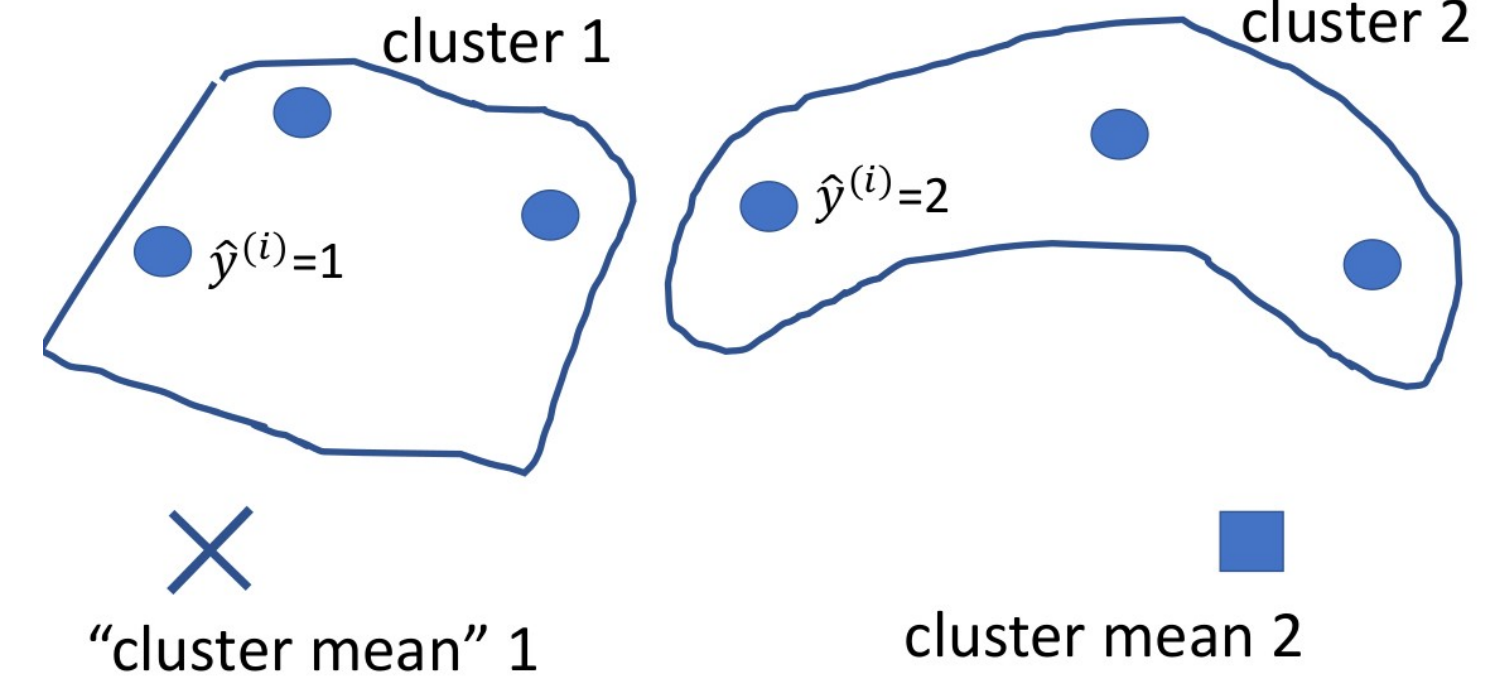
\includegraphics[scale=0.3]{images/CL/CL1.png}
    \caption{Caption}
    \label{fig:enter-label}
\end{figure}

We can measure the cluster spread through Average squared Euclidean distance between points and mean of cluster $ C^{(i)}$ :\\
Spread for a cluster: $ \dfrac{1}{|C^{(i)}|}  \sum\limits_{i\in C^{(i)}}^m || m^{(i)} - x^{(i)}||^2$ \\
Error in general with all the k cluster: $ \dfrac{1}{m} \sum\limits_{c=1}^k \sum\limits_{i \in C^{(C)}} || m^{(c)} - x^{(i)}||^2$

For given cluster means, clustering error is minimized by assigning $i^{th}$ data point to cluster with \textbf{nearest cluster mean} and for given cluster assignments, clustering error is minimized by representing $c^{th}$ cluster by the cluster mean of feature vectors of its data points

\begin{figure}[H]
    \centering
    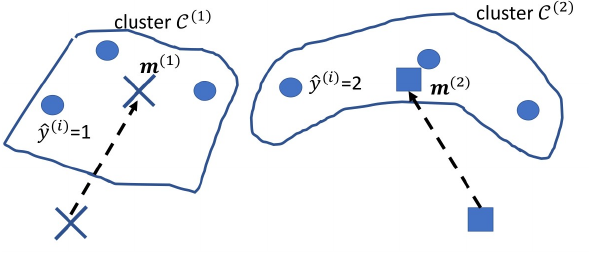
\includegraphics[scale=0.5]{images/CL/CL2.png}
    \caption{Caption}
    \label{fig:enter-label}
\end{figure}

The clustering error, to be minimized is an empirical risk minimization problem.\\
$ \epsilon ( \{ m^c \} , \{ \hat{y}^i \}) := \frac{1}{m} \sum\limits_{i=1}^m || m^{(\hat{y}^(i))} - x^{(i)}||^2  $\\
Simultaneously finding cluster means m(c) and assignments that minimize clustering error is difficult to complete, in fact it is NP-hard.
The solution is not solve the 2 problem together:
\begin{itemize}
    \item For given assignments, finding cluster means that minimize clustering error is easy
    \item  For given cluster means, finding assignments that minimize clustering error is easy
\end{itemize}

The cycle function will be like this:
\begin{enumerate}
    \item Input: number k of clusters, initial cluster means
    \item update cluster assignments
    \item update cluster means
    \item Go to step 2 until finished
    \item Output: final cluster means
\end{enumerate}

An important rules is that we can't increase error in our cycles, the error can only decrease or be the same. But the initialization is very important because a bad initialization can converge into a local optimum but not the optimal clustering because we can have multiple minimum.

\begin{figure}[H]
    \centering
    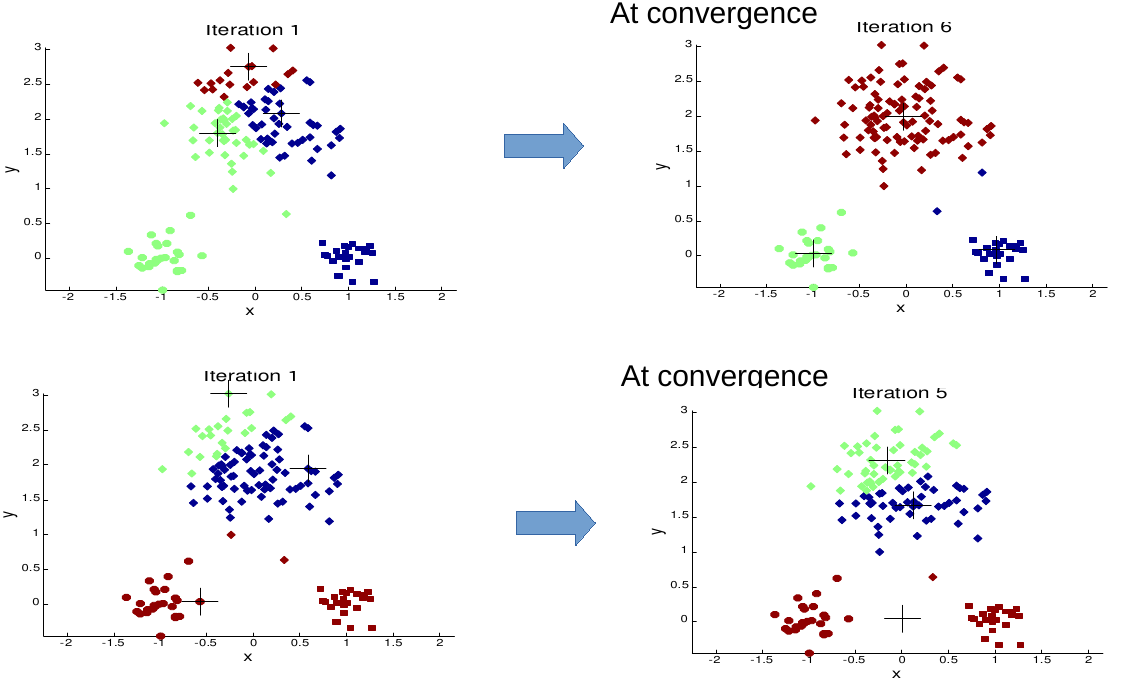
\includegraphics[scale=0.3]{images/CL/CL3.png}
    \caption{In the first image we have a good initialization in the second no}
    \label{fig:enter-label}
\end{figure}

To avoid that problem we can run some iteration with different initialization and choose the best; another problem could be choosing the k number of clusters and it could be done with the elbow method or given from the type of problem we have. Another method is to choose k by validation error with different value of k


\section{Soft clustering}
Indeed in soft clustering every datapoint is characterized by k label values, multilabel. Every value is a degree of the point belonging to cluster 1 to k. The value are between 0 and 1 and the results are a probability of being in a cluster or not.

\subsection{Gaussian mixture model}
 Each cluster produces data based upon random draws from a (multi-dimensional) Gaussian distribution and  should be less likely to have data at the edge, each Gaussian cluster has its own mean and standard deviation
\begin{figure}[H]
\centering
    \begin{subfigure}{.4\textwidth}
        \centering
        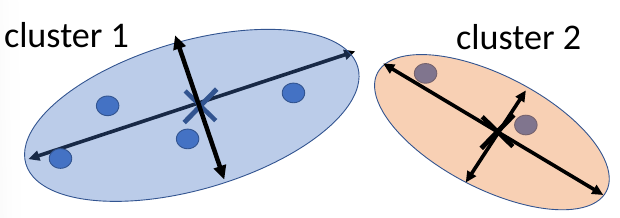
\includegraphics[width=1\linewidth]{images/CL/CL4.png}
        \caption{}
        \label{fig:sub1}
    \end{subfigure}
    \begin{subfigure}{.4 \textwidth}
        \centering
        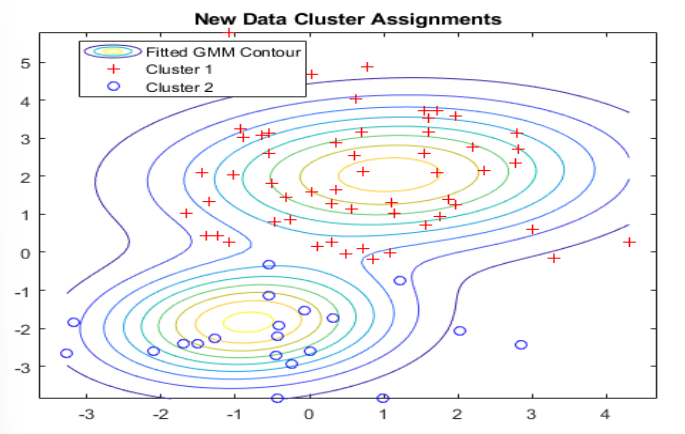
\includegraphics[width=1\linewidth]{images/CL/CL5.png}
        \caption{}
        \label{fig:sub1}
    \end{subfigure}
    \caption{}
\end{figure}
Mean vector: $ \mu$, covariance matrix $\Sigma$ \\
Gaussian distribution: $ \dfrac{e^{-\frac{1}{2} (x-\mu)^T \Sigma^{-1} (x-\mu )}}{\sqrt{(2\pi)^n det(\Sigma)}}$\\
Cluster spread: $\frac{1}{m^{(c)}} \sum\limits_{i=1}^m \hat{y}_c^i (x^i - \mu^c )^T  (\Sigma^1)^{-1} (x^i - \mu ^c) $\\
Means :$ \mu^c := \frac{1}{m^{(c)}} \sum\limits_{i=1}^m \hat{y}_c^i x^i $ for all c=1..k\\
Covariance: $\Sigma^C := \frac{1}{m^{(c)}}  \sum\limits_{i=1}^m  \hat{y}_c^i (x^i - \mu^c )^T (x^i - \mu ^c)$\\
Cluster assignment update: $  \hat{y}_c^i := \dfrac{m^c p(x^i| \mu^c , \Sigma^c )}{\sum\limits_{c'=1}^k m'^c p(x^i| \mu'^c , \Sigma'^c)} $


The algorithm is similar to the hard clustering updating in different moment in a loop until we resolve that.

\begin{itemize}
    \item INPUT: $(x^1, \dots , x^m), k, \{ \mu^c, \Sigma^c, m^c \} $
    \begin{enumerate}
        \item  Update soft cluster assignments $\hat{y}_c^i$
        \item Update cluster params $ \mu^c, \Sigma^c, m^c $
        \item Go to 1. unless “finished”
    \end{enumerate}
    \item OUTPUT: $\hat{y}_c^i, \mu^c, \Sigma^c, m^c $
\end{itemize}

The error: $ \epsilon := \sum\limits_{i=1}^m log \sum\limits_{c=1}^k  \frac{m^c}{m} p(x^i| \mu'^c , \Sigma'^c) $ This is negative logarithm of probability to sample data points under Gaussian mixture mode and it is equal to maximize likelihood; this is an Empirical Risk Minimization problem.

As in k-means we have the same problem about the initialization and the stop for cycle.
\subsection{Connectivity based clustering}
 k-Means and GMM fails on non-Euclidean cluster structure and cannot recognize outliers/noise. So we can use other types of clustering based on graph.  Connect close-by data points obtaining an empirical graph.
 This method use hard clustering and are 2:
 \begin{itemize}
     \item Spectral clustering: Eigenvectors of graph Laplacian matrix to measure connectivity between nodes
     \item DBSCAN: Density based spatial clustering with noise
 \end{itemize}

 \subsubsection{DBSCAN}
Data points need to be connected via core points, Core points are the ones with a minimum number of neighbors, Automatically determines number of k clusters. The outlier will be automatically discarded
It will accept 2 parameters:
\begin{itemize}
    \item Epsilon: Maximum distance to be connected
    \item MinPts: Minimum number of points to be a core point
\end{itemize}

\begin{figure}[H]
    \centering
    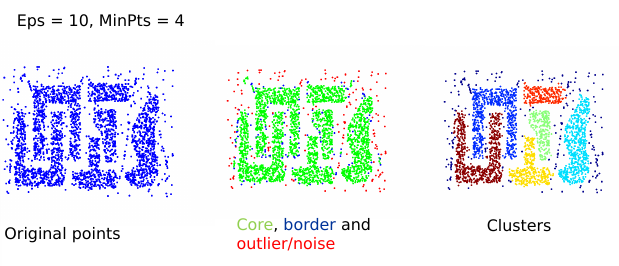
\includegraphics{images/CL/CL6.png}
    \caption{Caption}
    \label{fig:enter-label}
\end{figure}

\subsubsection{Hierarchical clustering}
A set of nested clusters organized as a hierarchical tree (dendogram); Any desired number of clusters can be obtained by ‘cutting’ the dendogram at the proper level and Different levels may correspond to meaningful taxonomies Key operation is the computation of the proximity of two clusters
\begin{figure}[H]
    \centering
    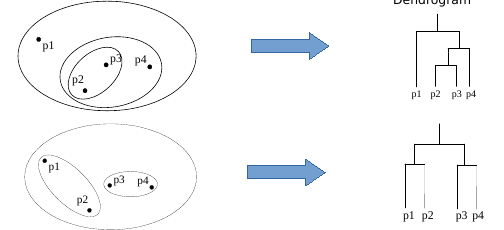
\includegraphics{images/CL/CL7.png}
    \caption{Caption}
    \label{fig:enter-label}
\end{figure}

\subsection{Comparing clustering}

We can measure a cluster validity using different index:
\begin{itemize}
    \item Internal Index: goodness of a clustering structure without external information (Ex: Silhouette index, sum of squared error (k-Means), log-likelihood)
    \item External or Relative Index: extent to which cluster labels match externally supplied class labels or labels from another clustering (Ex: entropy, purity, rand-index, adjusted rand-index, mutual information, adjusted mutual information)
\end{itemize}

\subsubsection{Silhouette index}
 Silhouette measures consistency within clusters of data: how similar a data point is to its own cluster (cohesion) compared to other clusters (separation). It is defined for each sample and is composed of two scores:
 \begin{itemize}
     \item The mean distance between a sample and all other points in the same cluster (a)
     \item The mean distance between a sample and all other points in the next nearest cluster (b)
 \end{itemize}
 \begin{center}
     $s= \dfrac{b-a}{max(a-b)}$
 \end{center}

It ranges from -1 to +1, where a high value indicates that the object is well matched to its own cluster and poorly matched to neighboring clusters, 0 indicate overlapping clusters.
High value are desired one and can be calculated with any distance metric.

The average silhouette over all data of a cluster measures how tightly grouped all the data in the cluster are

The average silhouette over all data of the dataset measures how appropriately the data has been clustered

\subsection{Rand Index}
Rand Index (RI) measures the similarity of two assignments and given a dataset D and two partitions S and R:\\
$RI(S,R) = \dfrac{a+b}{(\frac{m}{2})} \space (\frac{m}{2}) = \dfrac{m(m-1)}{2}$\\
where  a is the number of pairs of elements in D that are in the same subset in S and in the same subset in R and b is the number of pairs of elements in D that are in a different subset in S and in a different subset in R.Rand Index can be interpreted as accuracy but does not ensure to obtain a value close to 0.0 for a random labelling.

The adjusted Rand index corrects for chance and will give such a baseline:\\
$ ARI(S,R)= \dfrac{RI(S,R) - E [ RI ]}{max(RI) - E[RI]} $ \\
Max and expectation of RI are computed considering the number and size of clusters as in S and R, and all random clusterings are generated by shuffling the elements